\documentclass [a4paper] {article}
\usepackage[utf8]{inputenc}
\title{Ciencia de datos, práctica 5}
\author{Juan Casado Ballesteros, Samuel García Gonzalez, Iván Anaya Martín}
\usepackage{Sweave}
\begin{document}
\maketitle

\begin{abstract}
Realizaremos análisis de outliers sobre las dos muestrar proporcionadas según lo indicado en la práctica.
Para cada uno de los análisis realizados mostraremos los outliers obtenidos no solo de forma textual si no también con gráficos que nos ayuden a visualizar cada análisis.

Posteriormente hemos buscado un dataset que contiene medidas realizadas sobre los niveles de ozono, de temperatura, de humedad y de velocidad del viento.
Realizaremos el análisis de estos datos mediante regresión para lo cual primero realizaremos un análisis de outliers.
\end{abstract}

\newpage

\newpage
\section{Conocer los datos}
Cargamos y ostramos los datos que se nos han proporcionado para hacer la primera parte del ejercicio.

\subsection{Notas}
Los primeros datos representan la nota de laboratorio y de teorias evaluadas de 1 a 5.
\begin{Schunk}
\begin{Sinput}
> datos1 <- data.frame(read.table("datos1.txt"))
> datos1
\end{Sinput}
\begin{Soutput}
  Teoria Laboratorio
1      4           4
2      4           3
3      5           5
4      1           1
5      5           4
\end{Soutput}
\end{Schunk}
\begin{center}
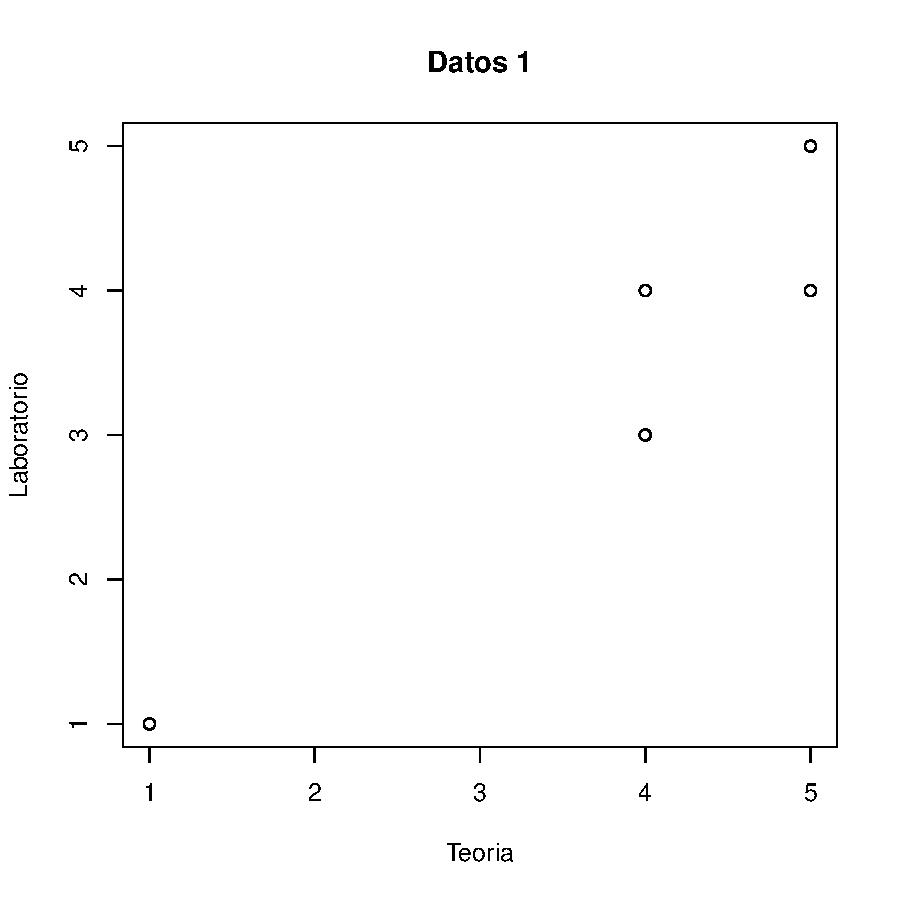
\includegraphics{entrega-plot_datos1}
\end{center}

\newpage
\subsection{Hormigón}
Los segundos representan la densidad y la resistencia del hormigón.
\begin{Schunk}
\begin{Sinput}
> datos2 <- data.frame(read.table("datos2.txt"))
> datos2
\end{Sinput}
\begin{Soutput}
  Resistencia Densidad
1         3.0      2.0
2         3.5     12.0
3         4.7      4.1
4         5.2      4.9
5         7.1      6.1
6         6.2      5.2
7        14.0      5.3
\end{Soutput}
\end{Schunk}
\begin{center}
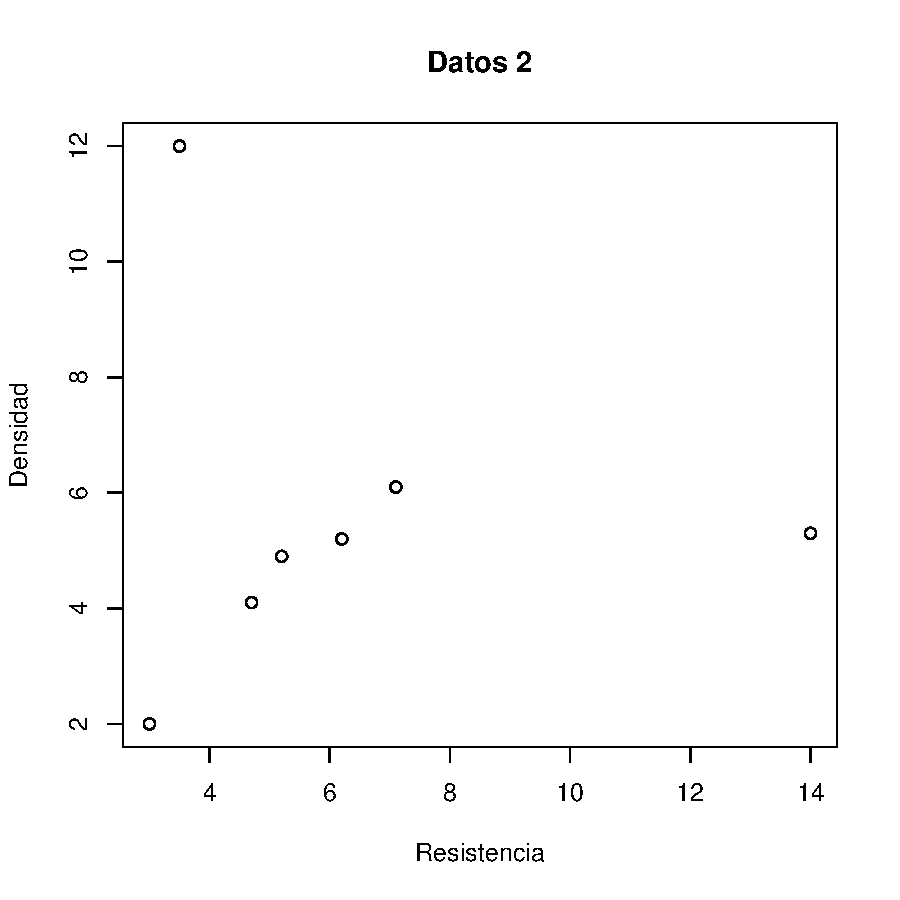
\includegraphics{entrega-plot_datos2}
\end{center}

\newpage
\section{K-vecinos sobre la muestra proporcionada para obtener outliers}
Aplicaremos el algoritmo k-vecinos sobre la muestra que tenemos.
Este algoritmo identificará de forma supervisada en la muestra datos anómalos, para poder obtener los outliers.

Calculamos las distancias euclídeas entre todos los puntos.
\begin{Schunk}
\begin{Sinput}
> distancias <- as.matrix(dist(datos1))
> distancias
\end{Sinput}
\begin{Soutput}
         1        2        3        4        5
1 0.000000 1.000000 1.414214 4.242641 1.000000
2 1.000000 0.000000 2.236068 3.605551 1.414214
3 1.414214 2.236068 0.000000 5.656854 1.000000
4 4.242641 3.605551 5.656854 0.000000 5.000000
5 1.000000 1.414214 1.000000 5.000000 0.000000
\end{Soutput}
\end{Schunk}

Elegimos el grado a partir del cual consideraremos que un pounto es outlier.
Todos los valores cuyo tercer vecino más cercano esté a una distancia superior a 2.5 los consideraremos outliers.
\begin{Schunk}
\begin{Sinput}
> max_radio <- 2.5
\end{Sinput}
\end{Schunk}

Mostramos en torno a cada valor un círculo con el radio indicado.
Si dentro del círculo dibujado no hay al menos otros tres datos dicho valor será considerado outlier.
Podemos ver que solo hay un punto para el que se da esta condición.
\begin{center}
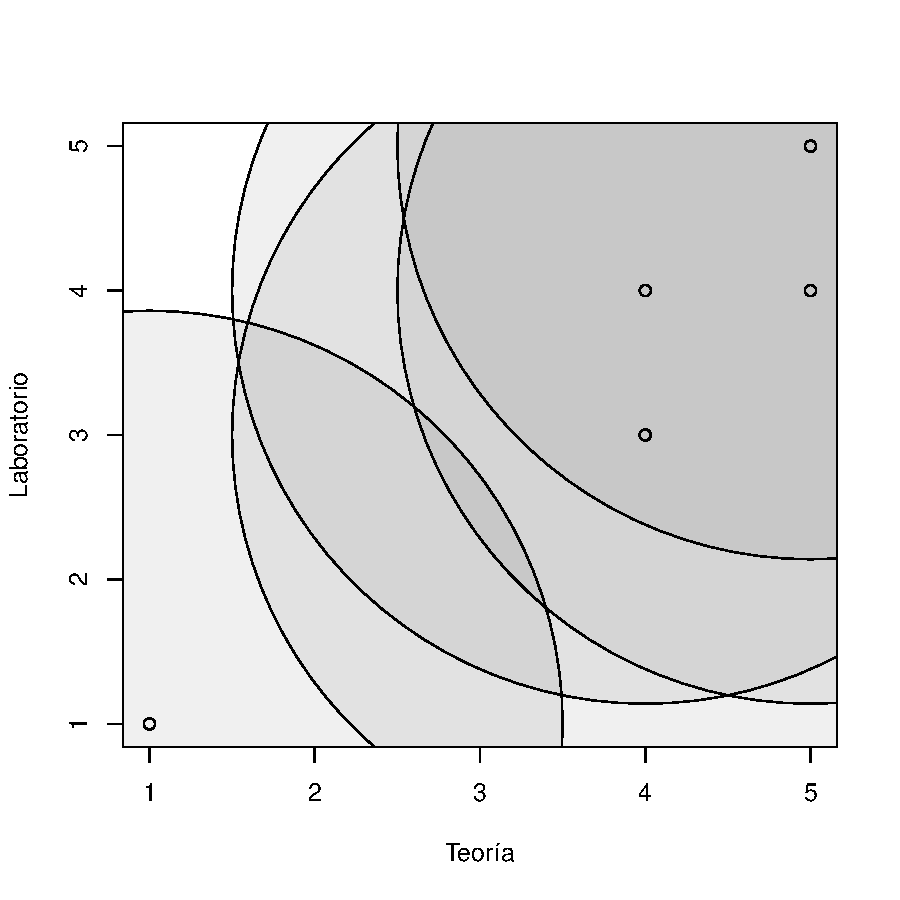
\includegraphics{entrega-k_vecinos_plot}
\end{center}

Calcularemos numéricamente ese valor.

Ordenamos las distancias de cada punto a todos los demás.
\begin{Schunk}
\begin{Sinput}
> for(i in 1:length(distancias[,1])){
+   distancias[,i] <- sort(distancias[,i])
+ }
> distanciasordenadas <- distancias
\end{Sinput}
\end{Schunk}

Reordenamos la matriz para organizarla en función de la distancia de cada punto a su vecino número 1,2,3...etc. 
Tras haber organizado la matriz, buscamos en el tercer vecino, que es el valor k que hemos usado en nuestro análisis para poder identificar los outliers.
\begin{Schunk}
\begin{Sinput}
> outliers_kvecinos = list()
> for(i in 1:length(distanciasordenadas[,1])){
+   if(distanciasordenadas[4,i]>max_radio){
+     outliers_kvecinos[[length(outliers_kvecinos)+1]] <- datos1[i,]
+   }
+ }
> outliers_kvecinos
\end{Sinput}
\begin{Soutput}
[[1]]
  Teoria Laboratorio
4      1           1
\end{Soutput}
\end{Schunk}

\newpage
\section{Deteccion de datos anómalos por cuartiles}
Sobre el segundo set de datos eliminaremos utilizando el método de los cuartiles.

Elegiremos el fator por el que multiplicar Q3-Q1.
Todos los valores que se alegen esa distancia de Q1 hacia los negativo o de Q3 hacia los positevos serán considerados outliers.
\begin{Schunk}
\begin{Sinput}
> max_range = 1.5
\end{Sinput}
\end{Schunk}

\subsection{Resistencia del hormigón}
Mostramos el diagrama de caja y bigotes de la resistencia.
\begin{center}
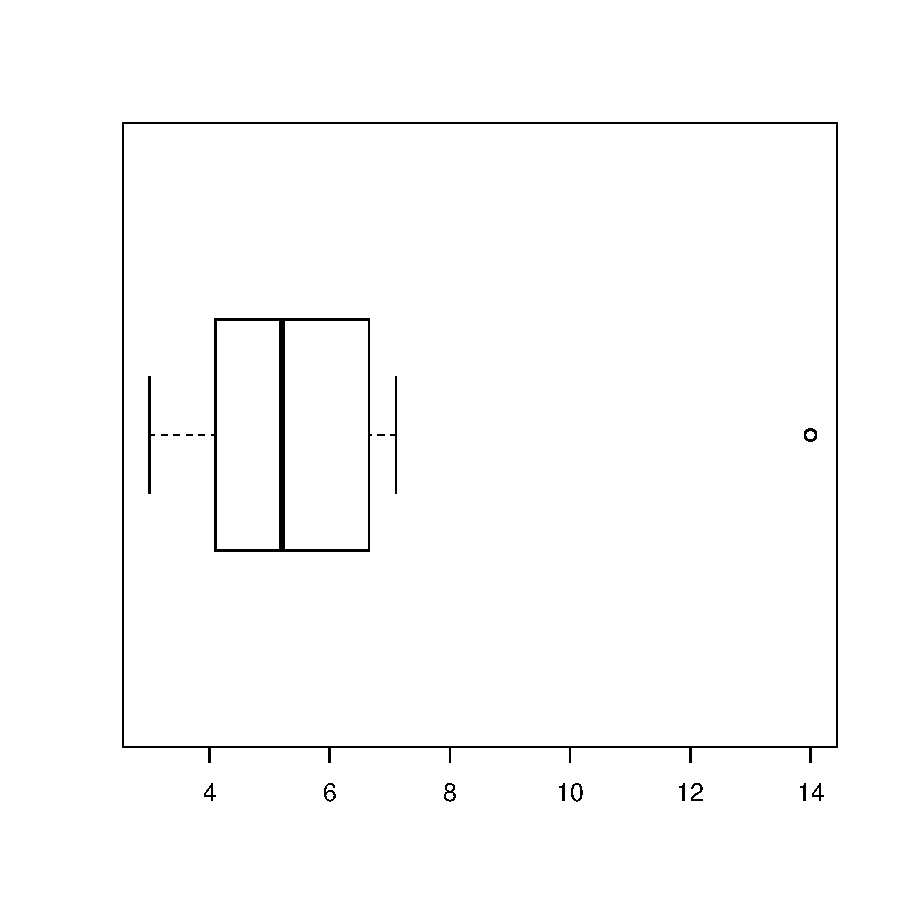
\includegraphics{entrega-plot_caja_bigotes_resistencia}
\end{center}

Calculamos ahora los valores que se salen del rango definido y que por tanto son outliers.
Para hacer esto primero obtenemos el intercalo de valores válidos
\begin{center}
\begin{Schunk}
\begin{Sinput}
> cuart1_res<-quantile(datos2$Resistencia,0.25)
> cuart3_res<-quantile(datos2$Resistencia,0.75)
> int_res=c(cuart1_res-max_range*(cuart3_res-cuart1_res),
+           cuart3_res+max_range*(cuart3_res-cuart1_res))
> int_res
\end{Sinput}
\begin{Soutput}
   25%    75% 
 0.275 10.475 
\end{Soutput}
\end{Schunk}
Ahora obtendremos los valores que quedan fuera de dicho intervalo.
\begin{Schunk}
\begin{Sinput}
> outliers_cuartiles_resistencia = list()
> for(i in 1:length(datos2$Resistencia)){
+   if(datos2$Resistencia[i]<int[1]||datos2$Resistencia[i]>int[2]){
+     outliers_cuartiles_resistencia[[length(outliers_cuartiles_resistencia)+1]] <- 
+         t(matrix(c(i, datos2[i,]$Resistencia), dimnames=list(c("Indice","Resistencia"))))
+   }
+ }
> outliers_cuartiles_resistencia
\end{Sinput}
\begin{Soutput}
[[1]]
     Indice Resistencia
[1,]      7          14
\end{Soutput}
\end{Schunk}
\end{center}
Como vemos el valor 12 es un outlier de la variable resistencia.

\subsection{Densidad del hormigón}
Repetimos este mismo análisis para la densidad.

Primero mostramos el diagrama de caja y bigotes para esta variable.
\begin{center}
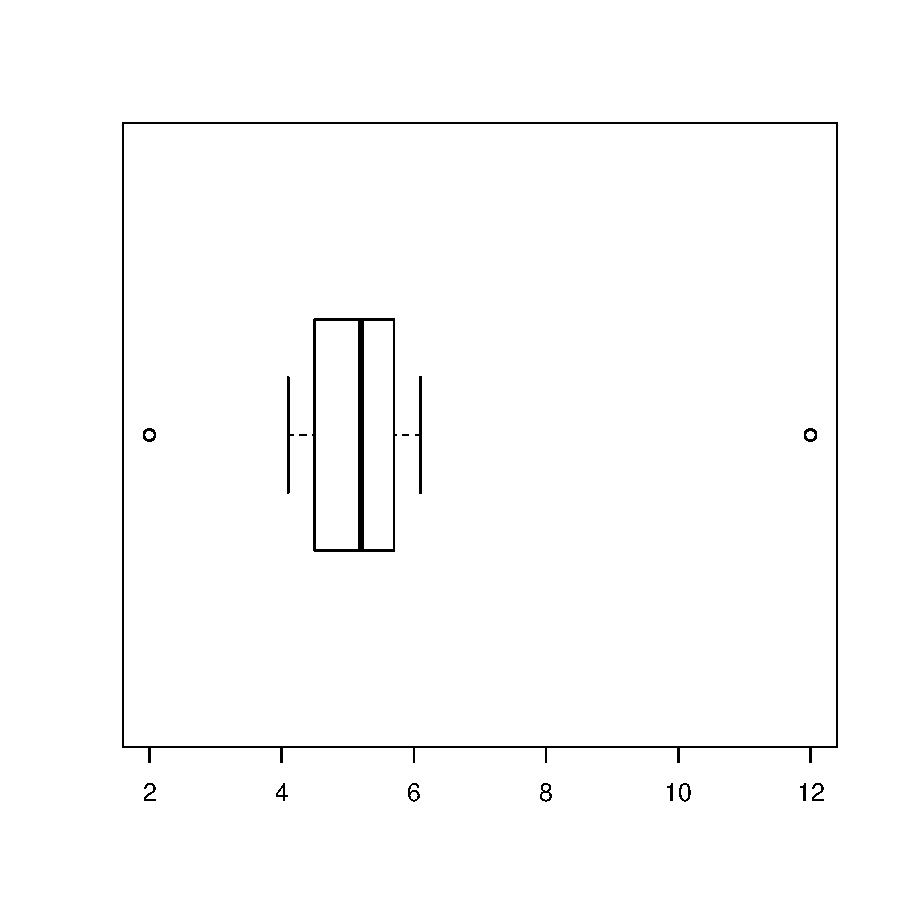
\includegraphics{entrega-plot_caja_bigotes}
\end{center}

Calculamos el intervalo a partir del que consideramos que los datos son outliers.
\begin{Schunk}
\begin{Sinput}
> cuart1_den<-quantile(datos2$Densidad,0.25)
> cuart3_den<-quantile(datos2$Densidad,0.75)
> int=c(cuart1_den-max_range*(cuart3_den-cuart1_den), 
+       cuart3_den+max_range*(cuart3_den-cuart1_den))
> int
\end{Sinput}
\begin{Soutput}
25% 75% 
2.7 7.5 
\end{Soutput}
\end{Schunk}

Obtenemos lo datos que quedan fuera del intervalo.
\begin{Schunk}
\begin{Sinput}
> outliers_cuartiles_densidad <- list()
> for(i in 1:length(datos2$Densidad)){
+   if(datos2$Densidad[i]<int[1]||datos2$Densidad[i]>int[2]){
+     outliers_cuartiles_densidad[[length(outliers_cuartiles_densidad)+1]] <- 
+       t(matrix(c(i, datos2[i,]$Densidad), dimnames=list(c("Indice","Densidad"))))
+   }
+ }
> outliers_cuartiles_densidad
\end{Sinput}
\begin{Soutput}
[[1]]
     Indice Densidad
[1,]      1        2

[[2]]
     Indice Densidad
[1,]      2       12
\end{Soutput}
\end{Schunk}

Esta vez hay dos valores outlier de densidad el 2 y el 12.


\newpage
\section{Outliers mediante la desviación típica}
Calcularemos los valores para cada que son considerados outliers por el método de la desviación tipica.
Dichos valores serán aquellos que se alejen demasidado de la media de la variable analizada.

En primer lugar elegiremos el factor por el que multiplicar la desviación típica para generar el intervalo de valores no outliers entorno a la media.
Metiante el teorema de tchebychev sabemos que para un valor de 2 al menos el 75\% de los datos estarán dentro del intervalo generado.
\begin{Schunk}
\begin{Sinput}
> max_deviation = 2
\end{Sinput}
\end{Schunk}

\subsection{Densidad del hormigón}
Mostramos la frecuencia realativa de la densidad del hormigón con respecto a la media de esta magnitud en azul.
En gris se muestra el intervalo a partir del cual los valores que queden fuera de él son considerados outliers.
\begin{center}
\begin{Schunk}
\begin{Sinput}
> plotFrecuencyData(datos2$Densidad)
\end{Sinput}
\end{Schunk}
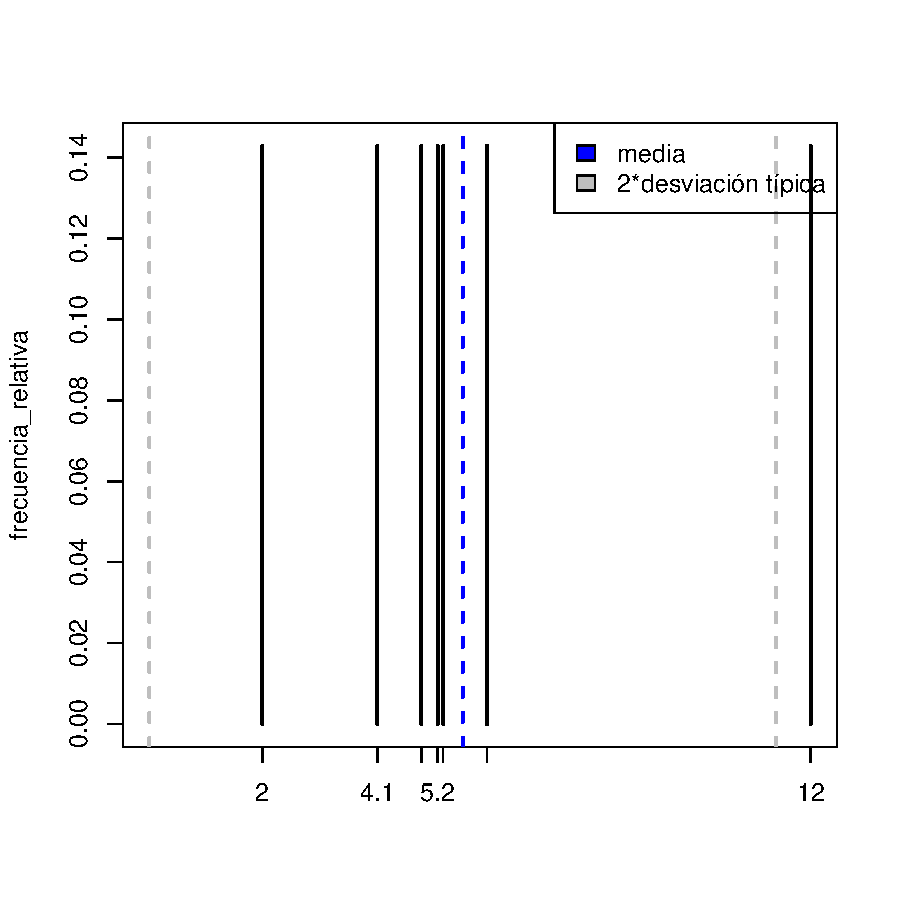
\includegraphics{entrega-desviacion_tipica_densidad_plot}
\end{center}

Ahora calculamos dichos valores.
Primero obtenemos el intervalo.
\begin{Schunk}
\begin{Sinput}
> int <- c(mediaAritmetica(datos2$Densidad) - 2*desviacionTipica(datos2$Densidad),
+          mediaAritmetica(datos2$Densidad) + 2*desviacionTipica(datos2$Densidad))
> int
\end{Sinput}
\begin{Soutput}
[1] -0.05685714 11.37114285
\end{Soutput}
\end{Schunk}
Podemos ver que el intervalo contiene valores de densidad irreales, esta no podría ser negativa.
En un anális de datos realista deberíamos corregir esto consultando con alguien que sea experto en los datos que estemos analizando.
Y luego los valores que quedan fuera de él.
\begin{Schunk}
\begin{Sinput}
> outliers_desviacion = list()
> for(i in 1:length(datos2$Densidad)) {
+   if ((datos2$Densidad[i]<int[1]) || (datos2$Densidad[i]>int[2])) {
+     outliers_desviacion[[length(outliers_desviacion)+1]] <- 
+       t(matrix(c(i, datos2[i,]$Densidad), dimnames=list(c("Indice","Densidad"))))
+   }
+ }
> outliers_desviacion
\end{Sinput}
\begin{Soutput}
[[1]]
     Indice Densidad
[1,]      2       12
\end{Soutput}
\end{Schunk}

\subsection{Resistencia del hormigón}
Mostramos la frecuencia realativa de la resistencia del hormigón con respecto a la media de esta magnitud en azul.
En gris se muestra el intervalo a partir del cual los valores que queden fuera de él son considerados outliers.
\begin{center}
\begin{Schunk}
\begin{Sinput}
> plotFrecuencyData(datos2$Resistencia)
\end{Sinput}
\end{Schunk}
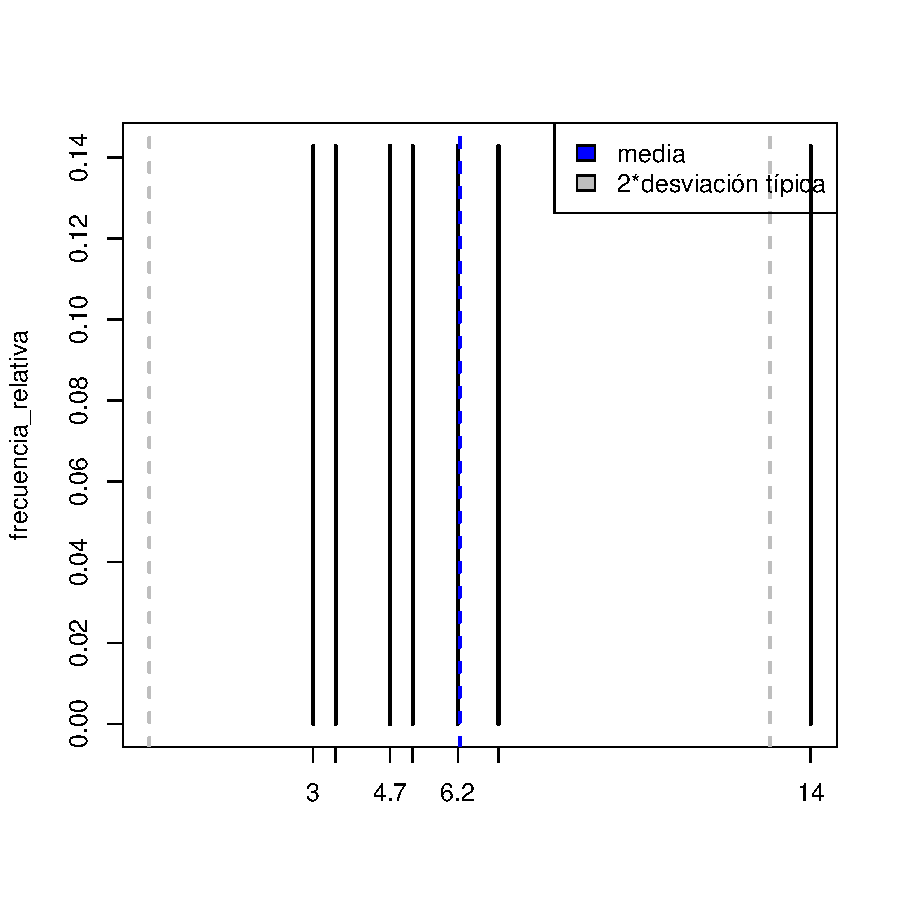
\includegraphics{entrega-desviacion_tipica_resistencia_plot}
\end{center}
Ahora calculamos dichos valores.
Primero obtenemos el intervalo.
\begin{Schunk}
\begin{Sinput}
> int <- c(mediaAritmetica(datos2$Resistencia) - 2*desviacionTipica(datos2$Resistencia), 
+          mediaAritmetica(datos2$Resistencia) + 2*desviacionTipica(datos2$Resistencia))
> int
\end{Sinput}
\begin{Soutput}
[1] -0.6197597 13.1054740
\end{Soutput}
\end{Schunk}
Podemos ver que el intervalo contiene valores de resistencia irreales, esta no podría ser negativa.
En un anális de datos realista deberíamos corregir esto consultando con alguien que sea experto en los datos que estemos analizando.
Y luego los valores que quedan fuera de él.
\begin{Schunk}
\begin{Sinput}
> outliers_desviacion = list()
> for(i in 1:length(datos2$Resistencia)) {
+   if ((datos2$Resistencia[i]<int[1]) || (datos2$Resistencia[i]>int[2])) {
+     outliers_desviacion[[length(outliers_desviacion)+1]] <- 
+       t(matrix(c(i, datos2[i,]$Resistencia), dimnames=list(c("Indice","Resistencia"))))
+   }
+ }
> outliers_desviacion
\end{Sinput}
\begin{Soutput}
[[1]]
     Indice Resistencia
[1,]      7          14
\end{Soutput}
\end{Schunk}

\newpage
\section{Detección de datos anómalos sobre la regresión de la densidad en función de la resistencia}

En este análisis detectamos los outliers utilizando la recta de regresión y el error estándar de los residuos.
Comenzaremos por determinar el factor por el que multiplicar el error estándar para considerar que los datos son outliers.
\begin{Schunk}
\begin{Sinput}
> sr_factor = 2
\end{Sinput}
\end{Schunk}

Comenzamos el análisis calculando la recta de regresión de los datos.
\begin{Schunk}
\begin{Sinput}
> dFr=lm(datos2$Densidad~datos2$Resistencia)
\end{Sinput}
\end{Schunk}

Posteriormente, obtenemos los residuos calculados a partir de la recta de regresión y el error estándar.
\begin{Schunk}
\begin{Sinput}
> res=summary(dFr)$residuals
> res
\end{Sinput}
\begin{Soutput}
         1          2          3          4          5          6          7 
-3.8427477  6.1858698 -1.6454482 -0.8168308  0.4919157 -0.4595958  0.0868370 
\end{Soutput}
\begin{Sinput}
> sr=sqrt(sum(res^2)/length(res))
> sr
\end{Sinput}
\begin{Soutput}
[1] 2.850242
\end{Soutput}
\end{Schunk}

A partir del error estándar y de la recta de regresión obtenida podremos mostrar los datos junto a su recta de regresión.
Paralela a dicha recta mostramos otras dos que marcan la frontera a partir de la que los valores se considerarán outliers.
En este caso solo se ve la recta paralela superior.
\begin{center}
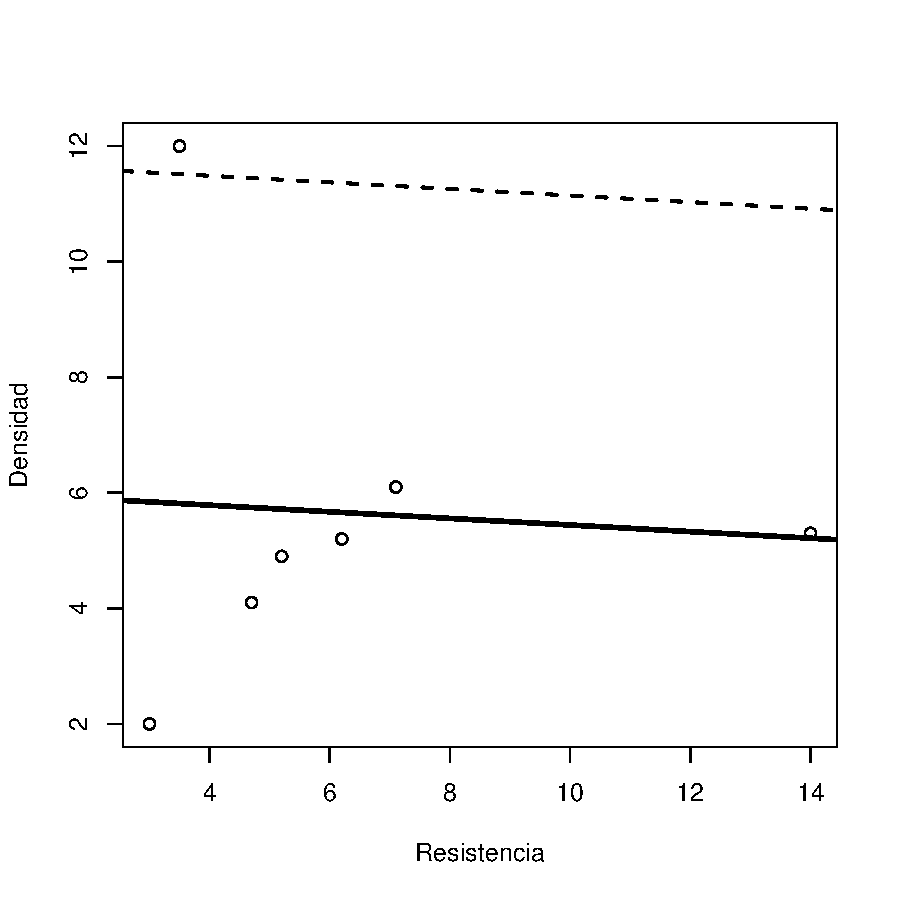
\includegraphics{entrega-regresion_plot}
\end{center}

Con el error estándar de los residuos, comparamos cada uno para comprobar si es mayor que el error estándar multiplicado por el factor establecido.
Si se da el caso, podemos considerar ese punto como un outlier.
\begin{Schunk}
\begin{Sinput}
> outliers_regresion = list()
> for(i in 1:length(res)){
+   if(abs(res[i])>sr_factor*sr){
+     outliers_regresion[[length(outliers_regresion)+1]] <- datos2[i,]
+   }
+ }
> outliers_regresion
\end{Sinput}
\begin{Soutput}
[[1]]
  Resistencia Densidad
2         3.5       12
\end{Soutput}
\end{Schunk}

\end{document}
